% ============================================================
% Sección 2
% ============================================================
\section{2 EDO de la forma $y'(x)=f(x)$}

\begin{tcolorbox}[enunciado]
Este es el caso más directo de aplicación del Teorema Fundamental del Cálculo visto en MCA1, simplemente debemos cuidar tomar un dominio donde la función $x'(t)$ tenga sentido, pues recuerde que la solución debe ser una función de clase $C^{1}$.

\vspace{0.2cm}
\textbf{Clases:}
\begin{itemize}[leftmargin=*]
    \item Isoclinas, Análisis Cualitativo 1 MCA4 2Sep26
\end{itemize}

\textbf{Documentación:}
\begin{itemize}[leftmargin=*]
    \item Notas: sobre la ecuación $y'(x)=f(x)$
\end{itemize}
\end{tcolorbox}

\subsection*{ACTIVIDADES}

\begin{enumerate}[label=\arabic*., leftmargin=*]
    \item \textbf{Evolución de la cola en un router}

    En un router, la longitud de la cola $q(t)$ aumenta con el tráfico entrante y disminuye con la capacidad de salida. Si la tasa de llegada supera la capacidad, la cola crece indefinidamente y puede desbordarse.

    Un modelo simplificado que lo representa es el siguiente:
    \[ \frac{d}{dt}q(t) = \frac{NW}{R} - C \]

    Donde:

    \vspace{0.3cm}
    \begin{center}
    \resizebox{\linewidth}{!}{
    \begin{tabular}{c p{9cm} c}
    \toprule
    \textbf{Constante} & \textbf{Significado} & \textbf{Unidades típicas} \\
    \midrule
    $q(t)$ & Longitud de la cola & paquetes (o bytes) \\
    \addlinespace
    $N$ & Número de flujos TCP activos que comparten el router (cuántas conexiones hay) & Adimensional (número de conexiones) \\
    \addlinespace
    $W$ & Tamaño promedio de la ventana de congestión TCP, i.e. cuántos paquetes puede enviar cada conexión antes de recibir un ACK & Paquetes \\
    \addlinespace
    $R$ & Tiempo de ida y vuelta (RTT) promedio (de un paquete) & Segundos (s) \\
    \addlinespace
    $C$ & Capacidad del enlace de salida del router. Es la velocidad máxima a la que el router puede transmitir paquetes por segundo & Paquetes por segundo ($\text{paq}/\text{s}$) \\
    \bottomrule
    \end{tabular}
    }
    \end{center}
    \vspace{0.3cm}

    $N, W, R, C$ son constantes positivas.
    \begin{itemize}[leftmargin=*]
        \item \textbf{Tasa de llegada:}
        \[ \lambda = \frac{NW}{R} \]
        con:
        \begin{itemize}[leftmargin=*]
            \item $\frac{W}{R}$: tasa de envío por conexión ($\text{paq}/\text{s}$).
            \item $\frac{NW}{R}$: tasa de llegada total al router ($\text{paq}/\text{s}$).
        \end{itemize}
    \end{itemize}

    Suponiendo que:
    \begin{itemize}[leftmargin=*]
        \item $N = 10$ flujos TCP
        \item $W = 5$ paquetes
        \item $R = 0.1\text{ s}$
        \item $C = 400\text{ paq}/\text{s}$
        \item y la condición inicial (ic) es: $q(0) = 0$.
    \end{itemize}

    Responde:
    \begin{enumerate}[label=(\alph*), leftmargin=*]
        \item ¿Qué significa TCP (en este contexto)?
        \subsection*{Solución}
        % Escribe tu respuesta aquí

        \item ¿Qué es un ACK y cómo está relacionado con el TCP? (Respuesta breve)
        \subsection*{Solución}
        % Escribe tu respuesta aquí

        \item ¿Cuál es la tasa de llegada?
        \subsection*{Solución}
        % Escribe tu respuesta aquí

        \item Encuentra $q(t)$ para la ic dada.
        \subsection*{Solución}
        % Escribe tu respuesta aquí

        \item ¿En qué tiempo se desborda la cola si $q_{\max} = Q = 20000$ paquetes?
        \subsection*{Solución}
        % Escribe tu respuesta aquí

        \item ¿Qué $C$ garantiza que nunca se desborde la cola?
        \subsection*{Solución}
        % Escribe tu respuesta aquí
    \end{enumerate}

    \item En la clase del 2 de Sep (vídeo) resolvimos la EDO:
    \[ y'(x) = x^{2} - 1 \]
    Responde:
    \begin{enumerate}[label=(\alph*), leftmargin=*]
        \item Da la solución analítica especificando su dominio.
        \subsection*{Solución}
        % Escribe tu respuesta aquí

        \item Si la condición inicial fuera $x_{0}=5$, $y(5)=3$, ¿cómo queda expresada la solución?
        \subsection*{Solución}
        % Escribe tu respuesta aquí

        \item ¿Se cumple el principio de existencia y unicidad?, es decir, ¿la solución existe y para una condición dada nunca se interseca con otra? Justifica gráficamente.
        \subsection*{Solución}
        % Escribe tu respuesta aquí
    \end{enumerate}

    \item Usando las notas, en la sección ``Generalizaciones. $f(x)$ no continua'' para el ejemplo:
    \begin{equation*}
        y'(x) = \frac{1}{\sqrt{|x|}(1-x)} \tag{1}
    \end{equation*}
    lee todo el desarrollo de su solución. Responde lo siguiente:
    \begin{enumerate}[label=(\alph*), leftmargin=*]
        \item ¿En qué valores presenta discontinuidades de salto?
        \subsection*{Solución}
        % Escribe tu respuesta aquí

        \item ¿En qué dominios queda definida la función derivada?
        \subsection*{Solución}
        % Escribe tu respuesta aquí

        \item Según el texto, ¿cuál es la conducta de las soluciones en cada dominio? (Sólo pon la conclusión que viene al final del análisis cualitativo general).
        \subsection*{Solución}
        % Escribe tu respuesta aquí

        \item Ya hemos visto que sea una solución de equilibrio o un punto donde no está definida la derivada, eso no implica forzosamente que una función solución que empieza en un punto fuera de ellas no pueda alcanzarlas. Para ver si las toca o no, se hace el análisis asintótico. \\
        Replica el análisis asintótico para este caso dado en el texto.
        \subsection*{Solución}
        % Escribe tu respuesta aquí

        \item Replica la solución analítica dada (cada intervalo da soluciones distintas).
        \subsection*{Solución}
        % Escribe tu respuesta aquí

        \item ¿Estas soluciones cumplen que son únicas?, es decir, nunca se intersecan entre ellas.
        \subsection*{Solución}
        % Escribe tu respuesta aquí

        \item Ya sabemos por el análisis asintótico que las funciones soluciones, como función continua, sí tocan la recta $x=0$. ¿Por qué la función continua por partes definida como:
        \[
        f(x) = \begin{cases} 
        -2\arctan(\sqrt{-x}) + C & \text{si } x \le 0 \\[8pt]
        \ln\left|\frac{1+\sqrt{x}}{1-\sqrt{x}}\right| + C & \text{si } 0 < x < 1 
        \end{cases}
        \]
        y cuya gráfica para $C=0$ se da en la figura (1) \textbf{NO ES SOLUCIÓN}?

        \begin{figure}[H]
            \centering
            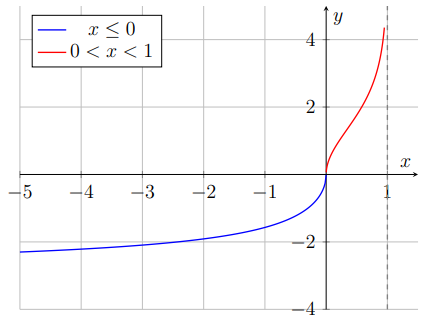
\includegraphics[width=0.45\linewidth]{imagenes/tarea/1figura.png}
            \caption{Gráfica de la función por partes con $C=0$}
        \end{figure}

        \subsection*{Solución}
        % Escribe tu respuesta aquí
    \end{enumerate}
\end{enumerate}